% Generated by pysimcount.pfseeds -- do not edit; regenerate instead.
% figure: B-order6-by-formula -- Every order-6 formula at measured r; median over seeds [1, 2, 3, 4, 5, 6, 7, 8, 9, 10], bars = min..max
% metric=t gatebase=ct merged
% seed 1: git_commit=01d3c275ceae2840002bd1aaea68f59b987c4975 git_dirty=False
% seed 2: git_commit=01d3c275ceae2840002bd1aaea68f59b987c4975 git_dirty=False
% seed 3: git_commit=01d3c275ceae2840002bd1aaea68f59b987c4975 git_dirty=False
% seed 4: git_commit=01d3c275ceae2840002bd1aaea68f59b987c4975 git_dirty=False
% seed 5: git_commit=01d3c275ceae2840002bd1aaea68f59b987c4975 git_dirty=False
% seed 6: git_commit=01d3c275ceae2840002bd1aaea68f59b987c4975 git_dirty=False
% seed 7: git_commit=01d3c275ceae2840002bd1aaea68f59b987c4975 git_dirty=False
% seed 8: git_commit=01d3c275ceae2840002bd1aaea68f59b987c4975 git_dirty=False
% seed 9: git_commit=01d3c275ceae2840002bd1aaea68f59b987c4975 git_dirty=False
% seed 10: git_commit=01d3c275ceae2840002bd1aaea68f59b987c4975 git_dirty=False
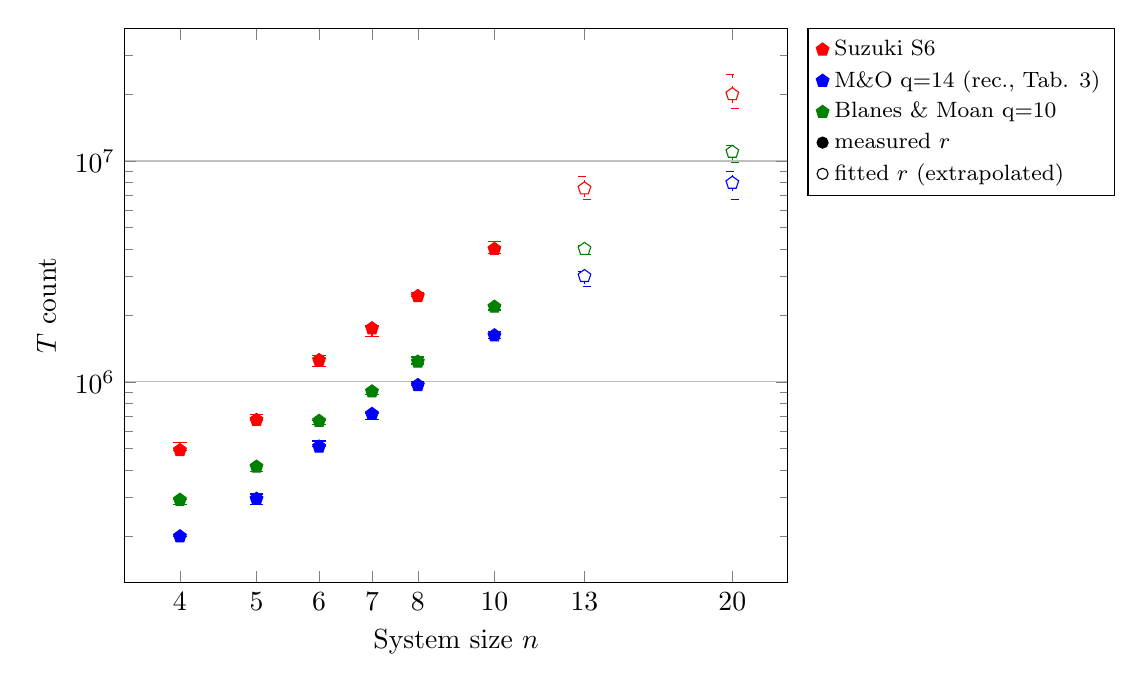
\begin{tikzpicture}
  \begin{loglogaxis}[
    width=10cm,
    xlabel={System size $n$},
    ylabel={$T$ count},
    xtick={4,5,6,7,8,10,13,20},
    xticklabels={4,5,6,7,8,10,13,20},
    ymajorgrids=true,
    legend pos=outer north east,
    legend cell align=left,
    legend style={font=\footnotesize},
  ]
    \addplot[only marks, red, mark=pentagon*, mark size=2.4pt, mark options={solid, fill=red}, error bars/.cd, y dir=both, y explicit, error bar style={red}] coordinates {
      (4,490685) += (0,40671) -= (0,1131)
      (5,672686) += (0,38464) -= (0,1442)
      (6,1254729) += (0,64127) -= (0,81529)
      (7,1747975) += (0,52889) -= (0,148923)
      (8,2446500) += (0,93082) -= (0,3420)
      (10,3997843) += (0,318145) -= (0,196833)
    };
    \addlegendentry{Suzuki S6}
    \addplot[only marks, red, mark=pentagon*, mark size=2.4pt, mark options={solid, fill=white}, forget plot, error bars/.cd, y dir=both, y explicit, error bar style={red, dashed}] coordinates {
      (13,7514691) += (0,974349) -= (0,801299)
      (20,20063997) += (0,4611641) -= (0,2718045)
    };
    \addplot[only marks, blue, mark=pentagon*, mark size=2.4pt, mark options={solid, fill=blue}, error bars/.cd, y dir=both, y explicit, error bar style={blue}] coordinates {
      (4,199740) += (0,60) -= (0,380)
      (5,295424) += (0,15496) -= (0,15672)
      (6,509056) += (0,30728) -= (0,1152)
      (7,715540) += (0,874) -= (0,40504)
      (8,966548) += (0,41496) -= (0,924)
      (10,1624174) += (0,64346) -= (0,53038)
    };
    \addlegendentry{M\&O q=14 (rec., Tab. 3)}
    \addplot[only marks, blue, mark=pentagon*, mark size=2.4pt, mark options={solid, fill=white}, forget plot, error bars/.cd, y dir=both, y explicit, error bar style={blue, dashed}] coordinates {
      (13,3012480) += (0,162468) -= (0,309312)
      (20,7963132) += (0,983748) -= (0,1234620)
    };
    \addplot[only marks, green!50!black, mark=pentagon*, mark size=2.4pt, mark options={solid, fill=green!50!black}, error bars/.cd, y dir=both, y explicit, error bar style={green!50!black}] coordinates {
      (4,292400) += (0,800) -= (0,13784)
      (5,413028) += (0,484) -= (0,20874)
      (6,665550) += (0,1102) -= (0,24126)
      (7,904662) += (0,19118) -= (0,28118)
      (8,1234038) += (0,61890) -= (0,28222)
      (10,2187862) += (0,28082) -= (0,70838)
    };
    \addlegendentry{Blanes \& Moan q=10}
    \addplot[only marks, green!50!black, mark=pentagon*, mark size=2.4pt, mark options={solid, fill=white}, forget plot, error bars/.cd, y dir=both, y explicit, error bar style={green!50!black, dashed}] coordinates {
      (13,3998210) += (0,160390) -= (0,224462)
      (20,10999812) += (0,781452) -= (0,1141124)
    };
    \addlegendimage{only marks, black, mark=*}
    \addlegendentry{measured $r$}
    \addlegendimage{only marks, black, mark=*, mark options={fill=white}}
    \addlegendentry{fitted $r$ (extrapolated)}
  \end{loglogaxis}
\end{tikzpicture}
